% Tal vez mencionar una descripción más extensa del resumen de cada capítulo. Mientras tanto puede quedar así 

\chapter{Marcos de trabajo}

% Este apartado se parece a una sección de los antecedentes. Creo que podría mover algo de eso por acá para hacer el repaso histórico de las herramientas 
% En este apartado se puede abordar la contradicción tecnológica 

% Antes este apartado se llamaba música algorítmica, supongo que quise retomar las discusiones sobre el uso amplio de estas plataformas es decir, fuera de supercollider

% Ejes fundamentales: programación eficiente y optimizada y otras búsquedas estéticas detrás del código.

% Encuentros en marcos restrictivos: restricción y ofrecimiento 

Este apartado hace referencias a reflexiones que resultaron del trabajo con marcos en la realización de piezas audiovisuales para el navegador. Cuando hablo de marcos me refiero a \gls{altonivel} como SuperCollider, OpenFrameworks, Three.js, Web Audio API entre otros. Si bien el caso de SuperCollider es particular, ya que es motor de audio, lenguaje de progrmación e intérprete al mismo tiempo, considero que marcos como los antes mencionados, guardan una relación abstracta con los motores que los posibilitan ( WebGL, OpenGL e incluso el servidor de SuperCollider como módulo independiente). Esto quiere decir que hay funciones sintetizadas que resuelven problemas específicos que no requieren una reconstrucción de bajo nivel. Dos ejes establecen el flujo de este capítulo:

\begin{itemize}

\item Las intenciones expresivas de programas escritos con lenguajes de programación y la contraposición entre la programación eficiente y optimizada y otro tipo de búsquedas como la ofuscación o el error.

\item El papel que juega la relación restricción y ofrecimiento como conceptos de la interacción humano-máquina (HCI), en la experienciación de los marcos de trabajo y la extensión a partir de funcionalidades básicas. 
  
\end{itemize}

% De manera paralela, se aborda el legado que hila el pensamiento musical algorítmico con las posibilidades de escribir módulos personalizados que permitan extender las posibilidades de motores y plataformas que ya existen y de esta forma, dar un giro personalizado a la expresividad del trabajo con audio e imagen. 

A continuación, relacionamos estos dos ejes con algunas descripciones técnicas de las piezas realizadas en conjunto con esta investigación, al mismo tiempo que las vinculamos con algunos de los marcos que se utilizaron en los distintos momentos de cada pieza.


%\end{multicols}
%\vspace*{\fill}
\begin{figure} 
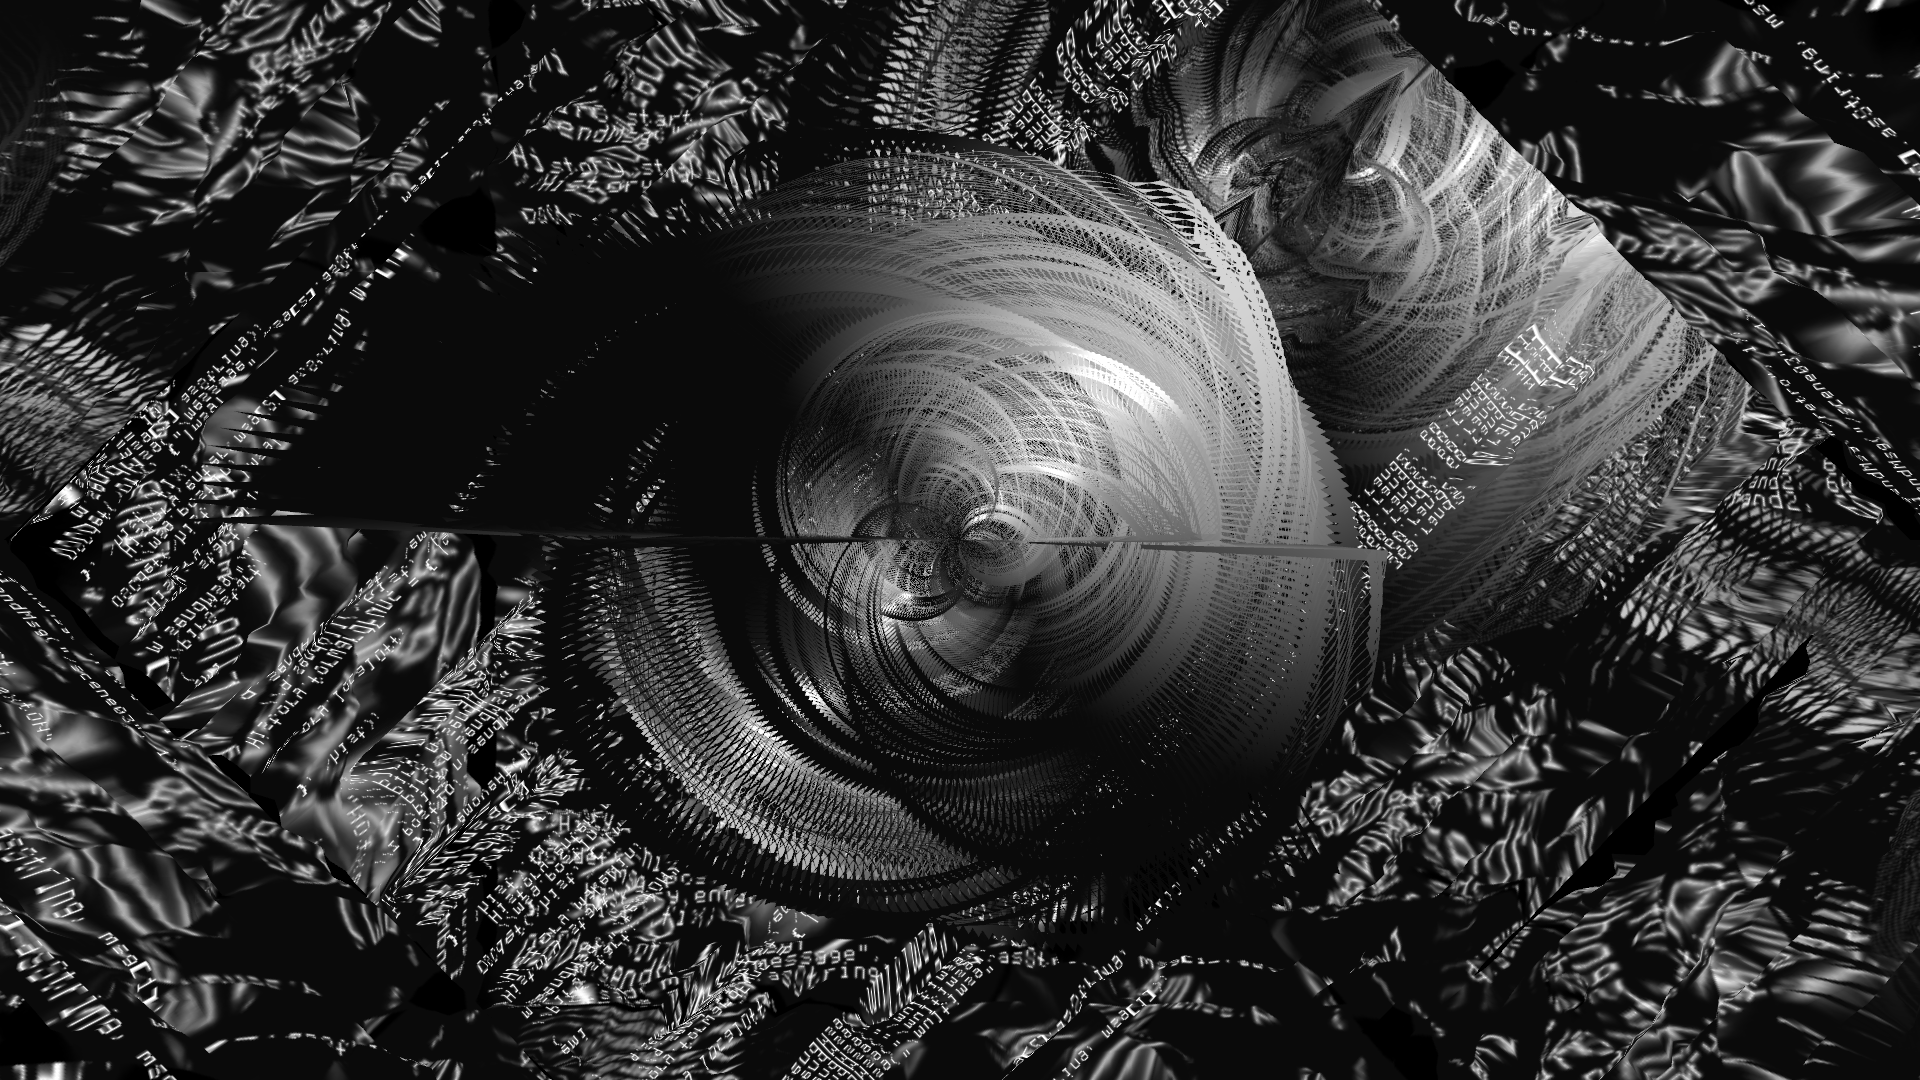
\includegraphics[width=\columnwidth]{../img/of13.png} 
\caption[Openframeworks 1]{Captura de render realizado con OpenFrameworks} % The text in the square bracket is the caption for the list of figures while the text in the curly brackets is the figure caption
\label{fig:gallery} 
\end{figure}

\clearpage
%\begin{multicols}{2}
  %\raggedright


%%%%%% Nombre pegador relacionado con alguna premisa de la descripción
%%%%%% 

%%%%%%%%%%%%%%%%%%%%%%%%%%%%%%%%%%%%%%%%%%%%%%%%%%%%%%%%%%%%%%%%
%%%%%%%%%%%%%%%%%%%%%%%%%%%%%%%%%%%%%%%%%%%%%%%%%%%%%%%%%%%%%%%%
%%%%%%%%%%%%%%%%%%%%%%%%%%%%%%%%%%%%%%%%%%%%%%%%%%%%%%%%%%%%%%%%

\section{La ofuscación como motivo}

Anti es una pieza que surgió como respuesta a tecnologías vinculadas con redes sociales como Instagram o Facebook. En específico, atiende a las tecnologías que permiten el diseño de experiencias, capas y filtros en Realidad Aumentada. En un conjunto de herramientas como la que ofrece Meta Spark ( antes llamado Spark AR), la personalización de las capas que se superponen a una imagen fija o en movimiento está determinada por una interfaz que acota las posibilidades de estas tecnologías al mismo tiempo que facilita su uso.

%\end{multicols}
%\vspace*{\fill}
\begin{Figure}
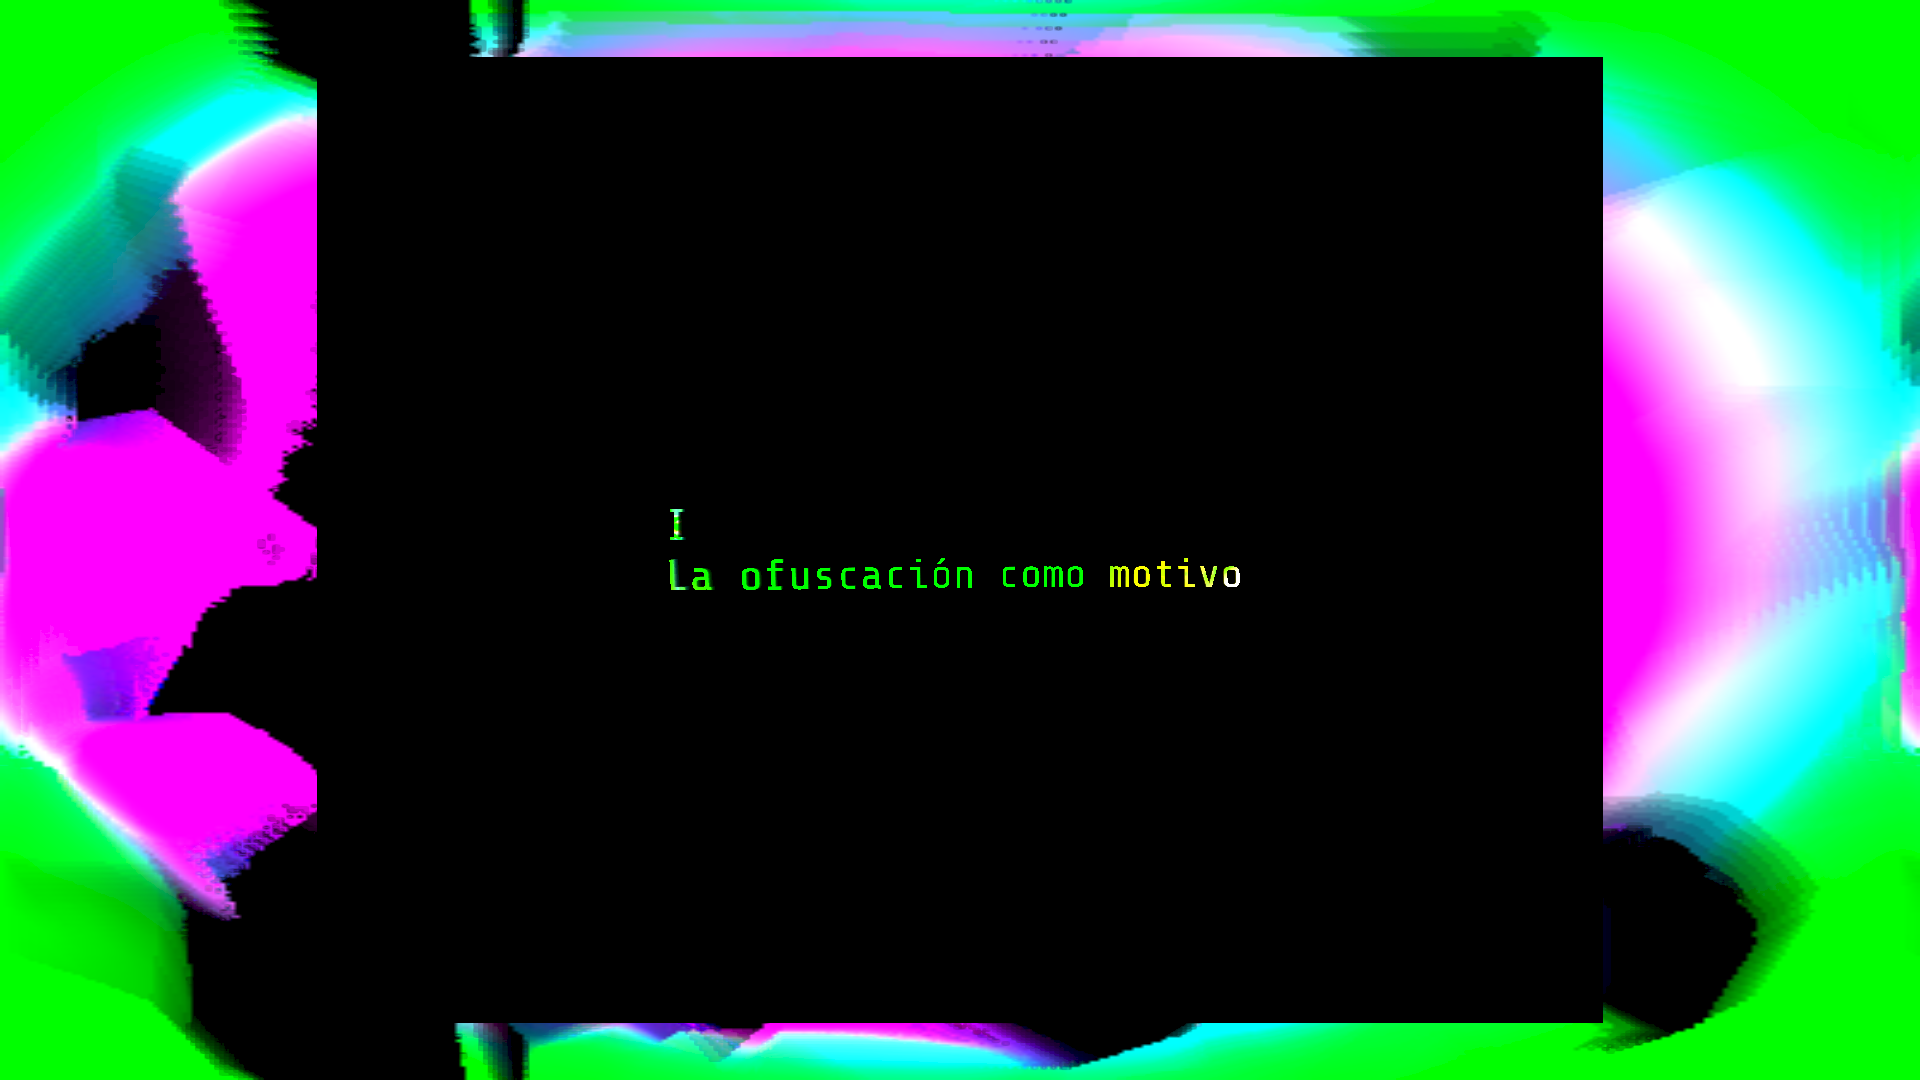
\includegraphics[width=\columnwidth]{../img/antiHydra1.png}
\captionof{figure}[Anti portada]{Portada del primer momento de Anti. La versión actual se puede consultar en: \url{https://anti.ocelotl.cc}.} % The text in the square bracket is the caption for the list of figures while the text in the curly brackets is the figure caption
\label{fig:gallery} 
\end{Figure}
%\clearpage
%\begin{multicols}{2}
  %\raggedright

Para la realización de Anti, tomé una decisión inicial que contemplaba tres caminos: el uso de Meta Spark, \Gls{openframeworks} o algún tipo de instancia para la web basada en P5.js o \Gls{threejs}.

Como parte del conjunto de restricciones que formaron parte de la intención inicial de este proyecto, Meta Spark quedó desacartada por ser una herramienta privativa. El uso de herramientas de software libre o código abierto puede ser muy ambiguo si consideramos que las licencias que sustentan estos estatutos tienen variaciones que por un lado pueden reforzar visiones optimistas pero poco efectivas en el campo profsional y que por otro, se adscriben a modelos que apoyan a proyectos o instancias con poca claridad en el manejo de datos como Facebook. Sin embargo, como parte de las decisiones subjetivas de este proyecto, considero que hay una frontera fundamental que se relaciona con una intención política pero también con una implicación de accesibilidad: experiencias que solamente pueden ser accedidas por medio de una red social, plataformas de creación de capas tipo filtro que solamente funcionan en un sistema operativo e incluso, la restricción que implica el uso de tarjetas gráficas dedicadas o cualquier tipo de escalada en los recursos físicos de la computadora o dispositivo desde el cual se accesa.

%\end{multicols}
%\vspace*{\fill}
\begin{Figure}
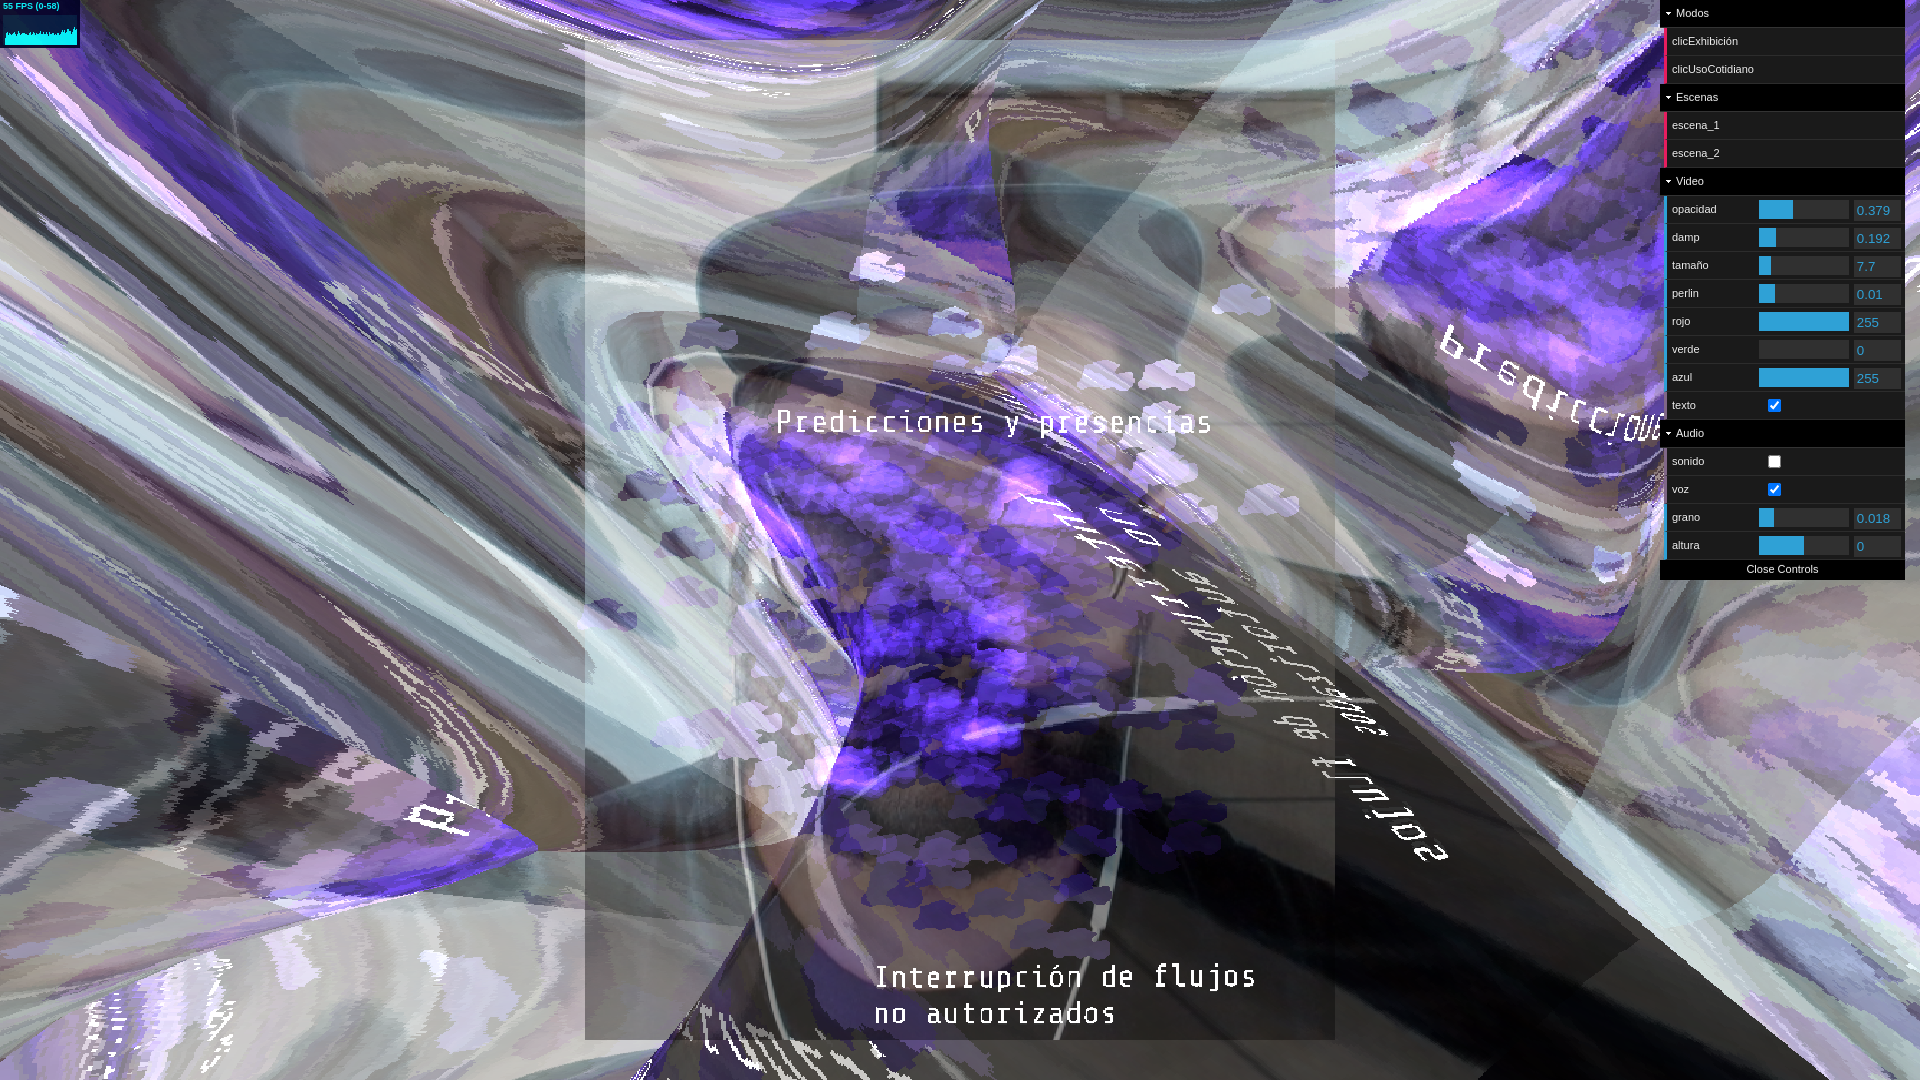
\includegraphics[width=\columnwidth]{../img/anti01.png}
\captionof{figure}[Anti]{Anti e interfaz gráfica. \url{https://anti.ocelotl.cc}.} % The text in the square bracket is the caption for the list of figures while the text in the curly brackets is the figure caption
\label{fig:gallery} 
\end{Figure}
%\clearpage
%\begin{multicols}{2}
  %\raggedright

  La premisa principal de Anti fue la exploración en términos visuales y sonoros del concepto ofuscación audiovisual de voz y rostro. El objetivo de la premisa tecnológica fue intervenir de alguna manera la cara que es capturada por una cámara y el audio que es registrado por un micrófono. Del lado del audio, no se utilizó algún tipo de análisis para transformar la voz, bastó con un filtro de granulación que permitiera modificar la voz sin que esta pudiera ser reconocible pero que pudiera seguir transmitiendo palabras entendibles por un escucha externo. Del lado de la imagen implementé un modelo de TensorFlow previamente entrenado de reconocimiento de puntos clave del rostro\footnote{El modelo específico que utilicé fue face-landmarks-detection. La colección de modelos se encuentra en: \url{https://github.com/tensorflow/tfjs-models}. Consultado el \today}. Hay tres ventajas de este modelo sobre de otros: la información no pasa por servidor externo, el modelo no busca detectar y diferenciar rostros y el nivel de precisión del modelo es bastante alto\citep{kartynnik2019realtime}.

  Como el modelo se ejecuta en Javascript, fue posible incorporarlo de una manera nativa a las librerías de renderado tridimensional y de audio. Eso generó un sistema relativamente eficiente e integrado que si bien no explora la ofuscación en términos del código mismo, si busca tener una intención en términos de la configuración de una herramienta tecnológica con un objetivo cotidiano como es ofuscar la información que se puede extraer del rostro y de la voz, sobre términos de la identificación, seguimiento y vigilancia del individuo. La ofuscación como motivo desdibuja la identidad para conservarla en un anonimato que puede ser compartido y que puede ser el prinicipio de otras formas de pensar la relación el humano como agente y el código como una tecnología imputada de un sentido que no solamente persigue la eficiencia.  

%\end{multicols}
\vspace*{\fill}
\begin{figure}
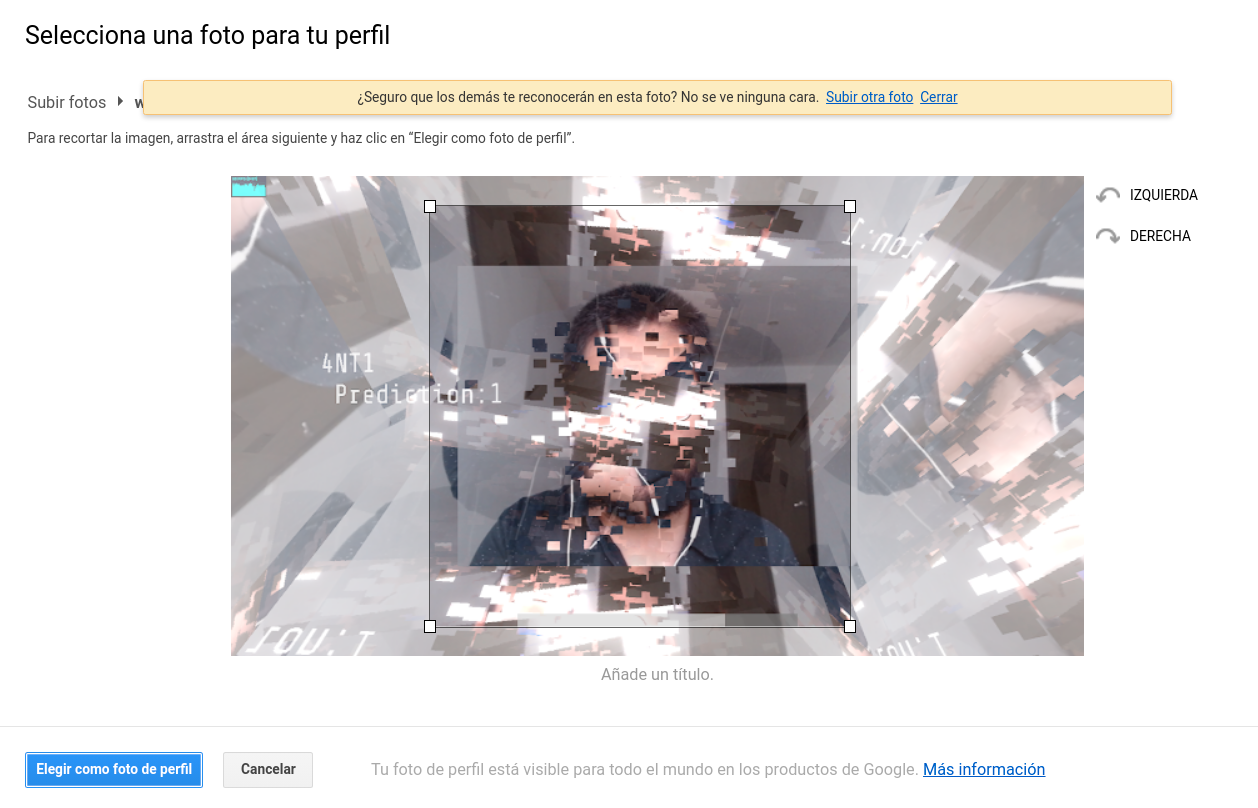
\includegraphics[width=\columnwidth]{../img/felicidades.png}
\captionof{figure}[Foto de perfil]{Captura de la primera imagen de Anti subida a Google como foto de perfil en la que no se reconoce el rostro.} % The text in the square bracket is the caption for the list of figures while the text in the curly brackets is the figure caption
\label{fig:gallery} 
\end{figure}
%\clearpage
%\begin{multicols}{2}
%\raggedright
  
Precisando en la discusión, la ofuscación puede definirse como el acto deliberado de encubrir el significado de una comunicación. Para el caso de la programación y apuntando ideas hacia los estudios del software, la presente investigación toma la noción de ofuscación de un conjunto de posibilidades para la escritura de software que coinciden, dialogan o se enfrentan a que podríamos definir como la convención de la \emph{estética del código} y aquellos programas que exploran ``otros principios estéticos'' además de los convencionales.

Edsger Dijkstra conoincide con la delimitación convencional de esta forma de escribir programas:

\begin{quote}
``[..] el programador no difiere de algún otro artesano: a menos de que ame sus herramientas, es altamente improbable que pueda crear algo de calidad superior. Al mismo tiempo estas consideraciones nos hablan de las más grandes virtudes que un programa puede mostrar: Elegancia y Belleza''\citep[p.~10]{EWD:EWD35}
\end{quote}

Como respuesta a la posición de Dijkstra y en un ámbito de programación que se aproxima lúdicamente a la escritura de programas, la ofuscación:

\begin{quote}
`` arroja luz a la naturaleza del código fuente, que es leído por un humano e interpretado por una máquina, y puede recordar a los críticos la búsqueda por diferentes dimensiones de sentido y múltiples codeos en todo tipo de programas''\citep[p.~198]{obfuscatedCode}
\end{quote}

El código su lectura, así como las funciones de los programas que ejecuta, son subjetivas y están determinadas por un sentido imputado que socialmente se acuerda de manera tácita y que puede ser visibilizado para interpelarlo en un sentido crítico, lúdico e incluso satírico.\footnote{Tal es el caso de Windows 93 del artista Jankenpopp. \url{https://www.windows93.net/} } En este punto encontramos conexiones con las posibilidades de la programación en una dimensión artística:

\begin{quote}
``[La práctica de la programación ofuscada] sugiere que el codeo puede resistir a la claridad y a la elegancia para pugnar en su lugar por la complejidad, puede hacer familiar lo desconocido y puede luchar con el lenguaje en el que está escrito, justo como lo hace la literatura contemporánea.''\citep[p.~198]{obfuscatedCode}
\end{quote}

La ofuscación puede definirse como el acto deliberado de encubrir el significado de una comunicación. Para el caso de la programación y apuntando ideas hacia los estudios del software, la presente investigación toma la noción de ofuscación de un conjunto de posibilidades para la escritura de software que coinciden, dialogan o se enfrentan a que podríamos definir como la convención de la \emph{estética del código} \citep{EWD:EWD35} y aquellos programas que exploran ``otros principios estéticos'' \citep{obfuscatedCode} además de los convencionales.

¿Puede el código fuente ``luchar'' en contra del marco de uso para el que fue escrito?

    
\section{Tres Estudios}

La práctica artística en contextos audiovisuales y performáticos que realicé hasta 2020 estuvo asociada al uso de SuperCollider para el audio y OpenFrameworks para el video. Las primeras aproximaciones a esta relación tecnológica se debió al trabajo realizado con Celeste Betancur, Jessica Rodríguez, Iracema de Andrade y Alejandro Brianza. Altamisa y Leviatán fueron dos piezas que implementaron esta relación y con apoyo de Celeste Betancur, fue posible realizar un sistema que pudiera detonar videos de acuerdo a decisiones que fueron controladas por medio del protocolo OSC. Esta relación fue ampliamente explorada y en particular, las relaciones y la composición centrada ya no únicamente en audio o video sino en flujos compartidos de información. Este eje continúa presente en la actualidad.

El tránsito de la relación SC y OF hacia Javascript fue motivado por las exigencias tecnológicas que implicó la transmisión de audio e imagen para espacios virtuales. El dominio tecnológico de una nueva herramienta puede suponer un reto y una curva de aprendizaje que requiere dedicación de tiempo. Consideramos que estas curvas pueden reducirse si en el proceso de escritura de código hay información sobre los antecedentes históricos y las ideas que conducen el funcionamiento fundamental de los marcos de trabajo. En este sentido, podemos realizar una observación comparativa entre la plataforma anteriormente utilizada (OF) y Three.js.

%\end{multicols}
%\vspace*{\fill}
\begin{figure}
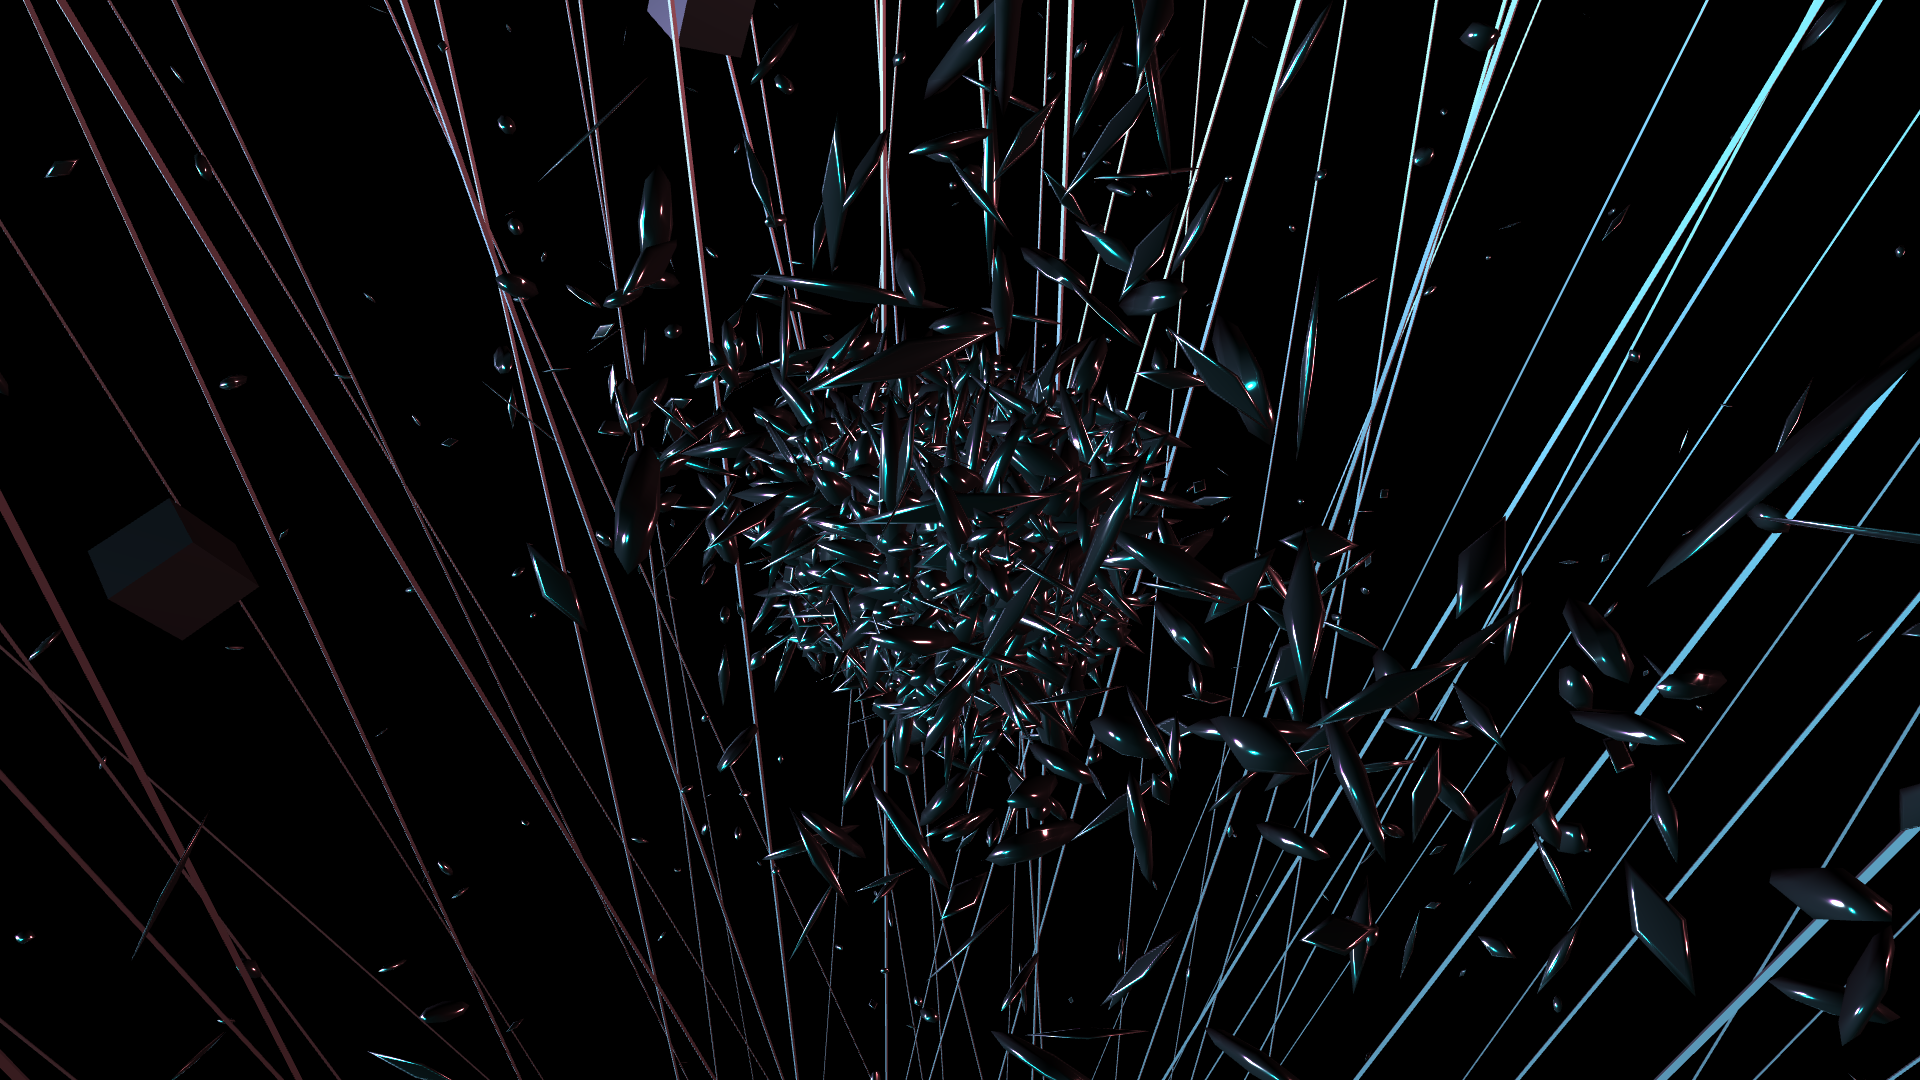
\includegraphics[width=\columnwidth]{../img/imagen2.png}
\captionof{figure}[THREE.studies]{Captura de la primera versión de THREE.studies} % The text in the square bracket is the caption for the list of figures while the text in the curly brackets is the figure caption
\label{fig:gallery} 
\end{figure}
\clearpage
%\begin{multicols}{2}

OpenFrameworks tiene una forma de concebir el espacio tridimensional, los objetos y las texturas de manera muy similar a Processing en tanto que son objetos que pueden ser invocados y se envuelven entre sí. Para el caso de Three.js, la aproximación se parece mucho más a la forma con la que se conciben los espacios y objetos tridimensionales en programas de diseño y modelado en tres dimensiones. En este sentido es posible trabajar de manera independiente con geometrías, materiales y mallas. 

Comparativa entre OpenFrameworks y Three.js. Estándares del trabajo con imagen que se heredan a través de Processing y que vienen de ideas más antiguas. 

El verdadero reto está en coinciliar los tiempos del audio y el video, siendo que cada uno corre en distintas tasas.

\section{La investigación compilada}

Como se mencionó en la introducción de esta investigación, este texto busca tener dos tipos de salidas: la primera es el texto fijado, impreso o en PDF y la segunda, una serie de recursos que giran en torno al texto y que pueden ser compiladas para el navegador web. 

\begin{comment}
El capitulo toma en consideración el estado actual de la relación entre música y lenguajes de programación como producto de una serie de ideas y perspectivas que han sido heredadas desde plataformas como Music N\citep{cambridgeElectronic} que derivan en interfaces delimitadas que interactúan con motores como SuperCollider o Chuck como Tidal Cycles\citep{mcleanTidal}

el rastreo histórico sobre la relación entre música y lenguajes de programación
Plataformas como Music N y el rastreo que hace Ge Wang sobre este tema.

\section{Legado Audio}

\subsection{Marcos de audio}

A continuación, haremos un breve rastreo de ideas centrales en la escritura de software orientado a la creación musical. El objetivo de este apartado consiste en describir y detectar la presencia del concepto unidad generadora en diversos programas orientados a la generación musical, de entre los cuales está una de las librerías que la presente investigación implementa.

El punto de partida de esta indagación es MUSIC N, proyecto de Max Mathews que sería el parteaguas del paradigma de la música por computadora. Uno de los primeros casos de esta instancia es el principio de programas como Max/MSP y PureData, proyectos representativos de la programación gráfica presente en flujos de trabajo gráfico actuales como TouchDesigner.

Como una observación adicional, es importante detectar instancias de la programación gráfica y de las ideas principales de la música por computadora en plataformas con giros programáticos particulares. Tal es el caso de OpenMusic, que de manera específica está basado en Common Lisp.

Desde la perspectiva de la programación escrita, destacamos el papel que ha tenido SuperCollider en la extensión del paradigma de la música por computadora en la actualidad. Señalamos la importancia de SuperCollider como el motor bajo el cual se pueden ejecutar entornos de programación al vuelo como Tidal Cycles o FoxDot. 

Estuary es un caso adicional que permite establecer un puente entre Tidal Cycles como un entorno que ejecuta SuperCollider como motor de audio y el navegador como tecnología multiplataforma sin instalaciones. Esta plataforma utiliza secuenciadores basados en la sintaxis de Tidal Cycles pero a diferencia del entorno que se puede instalar de manera local en una computadora, Estuary utiliza al navegador como motor de audio. 

Trazamos estas relaciones para establecer una relación continua y presente entre los entornos anteriormente descritos y una de las librerías utilizadas en los casos de estudio de esta investigación: Tone.js. En este sentido, consideramos importante la adscripción a los principios de la música por computadora para encontrar soluciones personalizadas para el navegador.


\subsection{Jacktrip y la música conectada}

Una parte de los antecdentes de este proyecto se vinculan con la actividad del colectivo RGGTRN\footnote{\url{https://rggtrn.github.io/}. Consultado el \today} y del LiveCodeNet Ensamble\footnote{\url{https://livecodenetensamble.wordpress.com/}. Consultado el \today}

RGGTRN es un colectivo de música por computadora fundado por Luis N. Del Angel y Emilio Ocelotl. Posteriormente se unieron Marianne Teixido y Jessica A. Rodríguez. Como parte de un ejercicio lúdico y de reflexión, el colectivo explora la improvisación audiovisual realizada por medio de código de programación, con una relación al contexto Latinx de sus participantes.

% Tesis de Luis
% Bellacode
% Saborítmico
% Tesis de maestría de hernani
% Artículo de Hernani en algún lado
% Artículos de Jessica ? 

raspis conectadas y jacktrip > el trabajo realizado por CCRMA y en general 

La labor del colectivo Radiador

% La radio y la transmisión de sonido con Icecast 

Sonobus y la resolución de problemas de streaming en tiempos de pandemia

\begin{itemize}
\item SuperCollider
\item CommonMusic 
\item Incluso plataformas de más alto nivel de lo que se trata en esta investigación como Megra, Tidal Cycles, Maximilian, Punctual o Conduct.
\item Max/MSP
\item WebAudioAPI
\item ¿DAWs? 
\end{itemize}

\section{Legado Video}

\subsection{Fluxus y openGL}

Para el caso de la imagen, retomo la influencia que tiene en la comunidad de live coding y en mi experienciación del performance audiovisual con la computadora el papel que tuvo el desarrollo Fluxus\footnote{\url{https://gitlab.com/nebogeo/fluxus/}} de Dave Griffiths que se remonta al 2007. Una característica peculiar de este desarrollo es el uso de una sintaxis tipo LISP que recuerda a desarrollos musicales basados en este lenguaje de programación como OpenMusic. 

Detrás de Fluxus también cabe destacar la importancia de sistemas de renderización de gráficos por computadora como OpenGL, que actualmente, son el punto de partida de software de alto nivel involucrado con este proyecto como OpenFrameworks y la variante para el navegador, webGL, que implementa la librería Three.js 

% Pregunta, esto no tendría que ir en otros momentos? Tal vez disperso o tal vez en la introducción 


\begin{itemize}
\item OpenFrameworks 
\item TouchDesigner y plataformas como 
\item Processing
\item Hydra
\item Three.js 
\end{itemize}

\section{El navegador como entorno intergrado} % Este apartado antes se llamada AV / Javascript

% Experiencia de Notas de Ausencia y de Panorama % Esto queda comentado, ya aparece en el apartado de antecedentes 

El anterior repaso da cuenta de los programas y plataformas que anteceden a esta investigación. Están enmarcadas en aplicaciones que se ejecutan localmente y que en ciertos casos, dependen directamente del sistema operativo en el que se ejecutan. A continuación, hablaremos del rumbo que tomó esta investigación hacia el navegador. Sobre este aspecto, destactamos dos resultados que articulan esta decisión:

\begin{itemize}
\item Estructuras compartidas fuera de un marco de trabajo como los que se han enunciado hasta el momento. Esto quiere decir que el navegador y el trabajo específico con Javascript permite organizar los motores gráficos y de audio en una estructura sin que esto requiera de algún tipo de protocolo de comunicación entre aplicaciones como OSC o MIDI.
\item Aplicaciones que corren en el navegador y que por este motivo, pueden ejecutarse prácticamente en cualquier sistema operativo con un navegador. Esto incluye a sistemas operativos para dispositivos móviles como iOS o Android. El coste de recursos es una limitación y la ausencia de un proceso de instalación podría ser una ventaja. % Revisar si esto ya está dicho 
\end{itemize}

% \section{Sistemas operativos y el navegador} % Estos dos módulos se pueden fundir, ojo con que no se descompensen los problemas
% No estoy muy seguro si aquí se pueden escribir las ideas de las secciones anteriores. Podría funcionar la reflexión sobre linux en esta parte? 
% EL papel que juegan las diferencias entre sistemas operativos, las aplicaciones multiplataforma. El navegador es una resolución a estas diferencias pero con un costo alto. % Esto ya estaba antes 
% El navegador como un sistema operativo entre sí (idea de Niklas Reppel). 

%%% Esto ya esta visible otra vez, quitar para la versión estable 

  La ofuscación puede definirse como el acto deliberado de encubrir el significado de una comunicación. Para el caso de la programación y apuntando ideas hacia los estudios del software, la presente investigación toma la noción de ofuscación de un conjunto de posibilidades para la escritura de software que coinciden, dialogan o se enfrentan a que podríamos definir como la convención de la \emph{estética del código} y aquellos programas que exploran ``otros principios estéticos'' además de los convencionales.

Edsger Dijkstra conoincide con la delimitación convencional de esta forma de escribir programas:

\begin{quote}
``[..] el programador no difiere de algún otro artesano: a menos de que ame sus herramientas, es altamente improbable que pueda crear algo de calidad superior. Al mismo tiempo estas consideraciones nos hablan de las más grandes virtudes que un programa puede mostrar: Elegancia y Belleza''\citep[p.~10]{EWD:EWD35}
\end{quote}

Como respuesta a la posición de Dijkstra y en un ámbito de programación que se aproxima lúdicamente a la escritura de programas, la ofuscación:

\begin{quote}
`` arroja luz a la naturaleza del código fuente, que es leído por un humano e interpretado por una máquina, y puede recordar a los críticos la búsqueda por diferentes dimensiones de sentido y múltiples codeos en todo tipo de programas''\citep[p.~198]{obfuscatedCode}
\end{quote}

El código su lectura, así como las funciones de los programas que ejecuta, son subjetivas y están determinadas por un sentido imputado que socialmente se acuerda de manera tácita y que puede ser visibilizado para interpelarlo en un sentido crítico, lúdico e incluso satírico.\footnote{Tal es el caso de Windows 93 del artista Jankenpopp. \url{https://www.windows93.net/} } En este punto encontramos conexiones con las posibilidades de la programación en una dimensión artística:

\begin{quote}
``[La práctica de la programación ofuscada] sugiere que el codeo puede resistir a la claridad y a la elegancia para pugnar en su lugar por la complejidad, puede hacer familiar lo desconocido y puede luchar con el lenguaje en el que está escrito, justo como lo hace la literatura contemporánea.''\citep[p.~198]{obfuscatedCode}
\end{quote}

La ofuscación puede definirse como el acto deliberado de encubrir el significado de una comunicación. Para el caso de la programación y apuntando ideas hacia los estudios del software, la presente investigación toma la noción de ofuscación de un conjunto de posibilidades para la escritura de software que coinciden, dialogan o se enfrentan a que podríamos definir como la convención de la \emph{estética del código} \citep{EWD:EWD35} y aquellos programas que exploran ``otros principios estéticos'' \citep{obfuscatedCode} además de los convencionales.

¿Puede el código fuente ``luchar'' en contra del marco de uso para el que fue escrito?

% Para la versión expandida podría citar las referencias 
% En este punto puedo retomar las ideas de djisktra y de knuth 

Esta definición es el punto de partida de \emph{Anti}, una pieza audiovisual para el navegador que tiene dos objetivos: visibilizar la discusión en torno a el uso de datos y la responsabilidad tecnológica del usuario y 2) actuar como un dispositivo de ofuscación facial y vocal que pueda utilizarse en situaciones de uso cotidiano. 

El maquillaje y el uso de accesorios anti-vigilancia son estrategias analógicas para evitar la detección de rostros. En una situación de protección fuera del entorno digital, incluso una máscara de leds puede cumplir esta función.

El presente proyecto se enfoca los mecanismos de anti-vigilancia que pueden realizarse de manera digital, teniendo a la computadora como un agente intermedio entre dos puntos que desean mantener algún tipo de comunicación gestual y vocal sin que estos puedan detectarse o asociarse a sujetos específicos, sin que esto implique que la comunicación sea completamente ofuscada para los usuarios.
\end{comment}
